%!TEX program = xelatex
%%%%%%%%%%%%%%%%%%%%%%%这是导言部分的开始%%%%%%%%

%========= 导言部分声明文档的类型=================
\documentclass{article}

	%=========导言部分可可以加载宏包=================
	\usepackage{amsmath}                % 数学公式排版宏包
	\usepackage{amssymb}                % 数学符号命令宏包
	\usepackage{amsthm}                 % 数学定理宏包
	\usepackage[UTF8]{ctex}             % 中文输入宏包
	\usepackage[a4paper]{geometry}      % 页面设置宏包
	\usepackage{setspace}               % 行间距宏包
	\usepackage{graphicx}               % 图片宏包
	\usepackage{listings}               % 代码宏包
	\usepackage{color}					% 颜色宏包
	\usepackage{xcolor}                 % 颜色处理宏包
	\usepackage{float}                  % 浮动对象式样宏包
	\usepackage{fontspec}
	
	%=========页面设置==============================
	\geometry{left=1cm,right=1cm,top=1cm,bottom=2cm}
	\onehalfspacing
	\setlength\parindent{0em}
	
	%=========代码格式设置============================
	\definecolor{dkgreen}{rgb}{0,0.6,0}
	\definecolor{gray}{rgb}{0.5,0.5,0.5}
	\definecolor{mauve}{rgb}{0.58,0,0.82}
	% \setmonofont{Consolas}
	\lstset{
		numbers = left, 	
		numberstyle = \color{gray}, 
		keywordstyle = \color{blue},
		commentstyle = \color{dkgreen}, 
		stringstyle = \color{mauve},
		basicstyle = \ttfamily,
		breaklines = true,
		frame = shadowbox, % 阴影效果
		rulesepcolor = \color{ red!20!green!20!blue!20} ,
		escapeinside = ``, % 英文分号中可写入中文
		xleftmargin = 2em,xrightmargin=2em, aboveskip=1em,
		framexleftmargin = 2em
	} 

%=========导言部分可以定义标题信息===============
\title{组会报告}
\author{徐益}
\date{2018/5/3}

%%%%%%%%%%%%%%%%%%%%%%%这是导言部分的结束%%%%%%%%%

%%%%%%%%%%%%%%%%%%%%%%%这是正文部分的开始%%%%%%%%%
\begin{document}
	
%=========生成标题================================
\maketitle

%=========开始正文的输入==========================

%===========第一节=================
\section{本周学习内容}

1. 多线程数据处理性能测试

2. DPDK添加方案

%===========第一节=================
\section{多线程数据处理性能测试}

\subsection{服务器运行运行信息}
\begin{figure}[H]
	\centering
	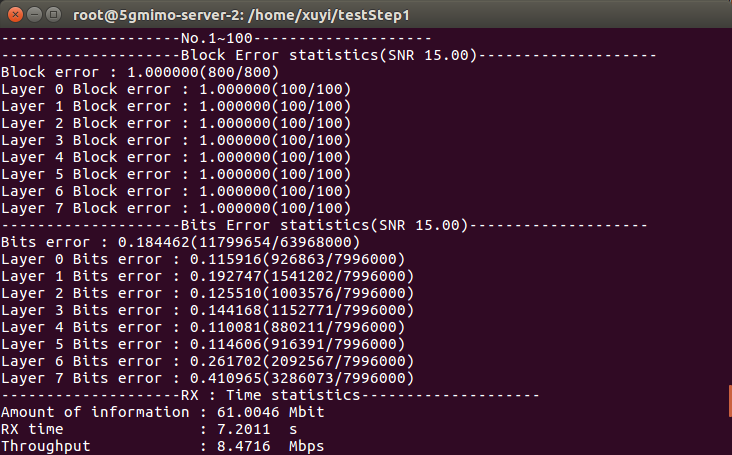
\includegraphics[width = .8\textwidth]{result_server.png}
	\caption{单台服务器处理信息(flowNum=8,CQI=15)}
\end{figure}

\subsection{不同CQI下的吞吐量}
\begin{table}[H]
\caption{不同CQI下的吞吐量(flowNum=8)}
\centering
\begin{tabular}{|l|l|l|l|}% 通过添加 | 来表示是否需要绘制竖线
	\hline  % 在表格最上方绘制横线
	CQI &	Modulation	&	TBS	&	Throughput	\\
	\hline
	1	&	QPSK		&	78	&	0.5729Mbps	\\
	\hline
	2	&	QPSK		&	120	&	0.8513Mbps	\\
	\hline
	3	&	QPSK		&	193	&	1.3445Mbps	\\
	\hline
	4	&	QPSK		&	308	&	2.0664Mbps	\\
	\hline
	5	&	QPSK		&	449	&	2.8582Mbps	\\
	\hline
	6	&	QPSK		&	602	&	3.6411Mbps	\\
	\hline
	7	&	16QAM		&	378	&	3.8403Mbps	\\
	\hline
	8	&	16QAM		&	490	&	4.7312Mbps	\\
	\hline
	9	&	16QAM		&	616	&	5.4568Mbps	\\
	\hline
	10	&	64QAM		&	466	&	5.7816Mbps	\\
	\hline
	11	&	64QAM		&	567	&	6.3868Mbps	\\
	\hline
	12	&	64QAM		&	666	&	7.1874Mbps	\\
	\hline
	13	&	64QAM		&	772	&	7.6519Mbps	\\
	\hline
	14	&	64QAM		&	873	&	8.0977Mbps	\\
	\hline
	15	&	64QAM		&	948	&	8.4716Mbps	\\
	\hline  % 在表格最下方绘制横线
\end{tabular}
\end{table}

%===========第二节=================
\section{DPDK添加方案}

\subsection{单服务器数据处理流程}
\begin{figure}[H]
	\centering
	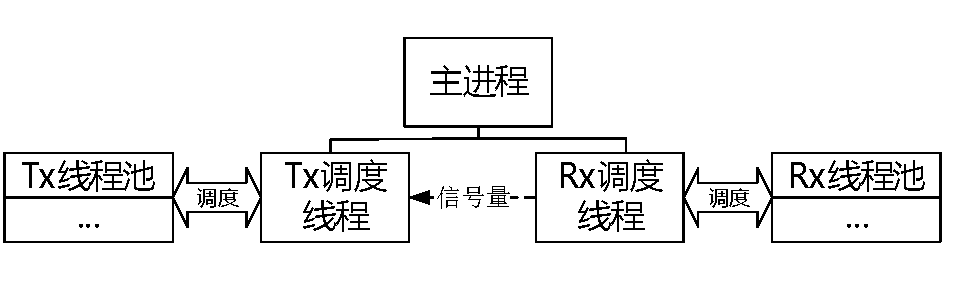
\includegraphics[width = \textwidth]{frame_step1.pdf}
	\caption{单服务器数据处理流程}
\end{figure}

\subsection{添加DPDK后的处理流程}
\begin{figure}[H]
	\centering
	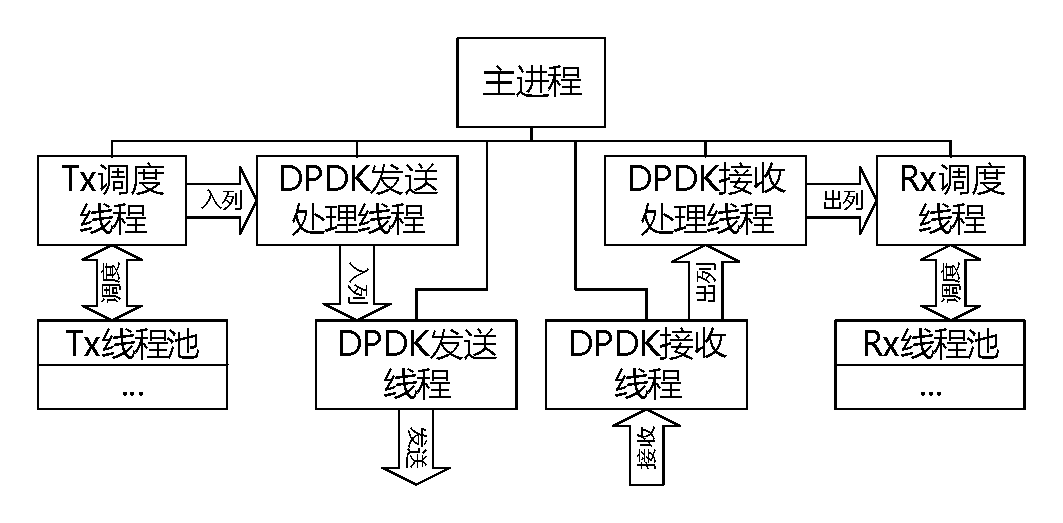
\includegraphics[width = \textwidth]{frame_step2.pdf}
	\caption{添加DPDK后的处理流程}
\end{figure}

%===========第三节=================
\section{DPDK}

%===========存在问题=================
\section{存在问题}
1. 

2. 

%===========下周计划=================
\section{下周计划}
1. 

2. 

\end{document}
%%%%%%%%%%%%%%%%%%%%%%%这是正文部分的结束%%%%%%%%%%%%